\documentclass[12t,letterpaper]{article}

\newenvironment{proof}{\noindent{\bf Proof:}}{\qed\bigskip}

\newtheorem{theorem}{Theorem}
\newtheorem{corollary}{Corollary}
\newtheorem{lemma}{Lemma} 
\newtheorem{claim}{Claim}
\newtheorem{fact}{Fact}
\newtheorem{definition}{Definition}
\newtheorem{assumption}{Assumption}
\newtheorem{observation}{Observation}
\newtheorem{example}{Example}
\newcommand{\qed}{\rule{7pt}{7pt}}

\newcommand{\assignment}[4]{
\thispagestyle{plain} 
\newpage
\setcounter{page}{1}
\noindent
\begin{center}
\framebox{ \vbox{ \hbox to 6.28in
{\bf Math 104: Introduction to Analysis \hfill #1}
\vspace{4mm}
\hbox to 6.28in
{\hspace{2.5in}\large\mbox{#2}}
\vspace{4mm}
\hbox to 6.28in
{{\it Handed Out: #3 \hfill Due: #4}}
}}
\end{center}
}

\newcommand{\solution}[3]{
\thispagestyle{plain} 
\newpage
\setcounter{page}{1}
\noindent
\begin{center}
\framebox{ \vbox{ \hbox to 6.28in
{\bf Math 104 \hfill #3}
\vspace{4mm}
\hbox to 6.28in
{\hspace{2.5in}\large\mbox{#2}}
\vspace{4mm}
\hbox to 6.28in
{#1 \hfill}
}}
\end{center}
\markright{#1}
}

\newenvironment{algorithm}
{\begin{center}
\begin{tabular}{|l|}
\hline
\begin{minipage}{1in}
\begin{tabbing}
\quad\=\qquad\=\qquad\=\qquad\=\qquad\=\qquad\=\qquad\=\kill}
{\end{tabbing}
\end{minipage} \\
\hline
\end{tabular}
\end{center}}

\def\Comment#1{\textsf{\textsl{$\langle\!\langle$#1\/$\rangle\!\rangle$}}}


\usepackage{amsmath, amssymb, dsfont}
\usepackage{graphicx}

\oddsidemargin 0in
\evensidemargin 0in
\textwidth 6.5in
\topmargin -0.5in
\textheight 9.0in
\newcommand{\norm}[1]{\left\lVert #1 \right\rVert}
\newcommand{\abs}[1]{\left\vert #1 \right\vert}
\newcommand{\?}{\stackrel{?}{=}}

\begin{document}

\solution{Nikhil Unni}{Assignment \#12}{Spring 2016}
\pagestyle{myheadings}

\begin{enumerate}
  \item [20.3]
    Repeat Exercise 20.1 for $f(x) = \frac{\sin x}{x}$. See Example 9 section 19.\\\\

    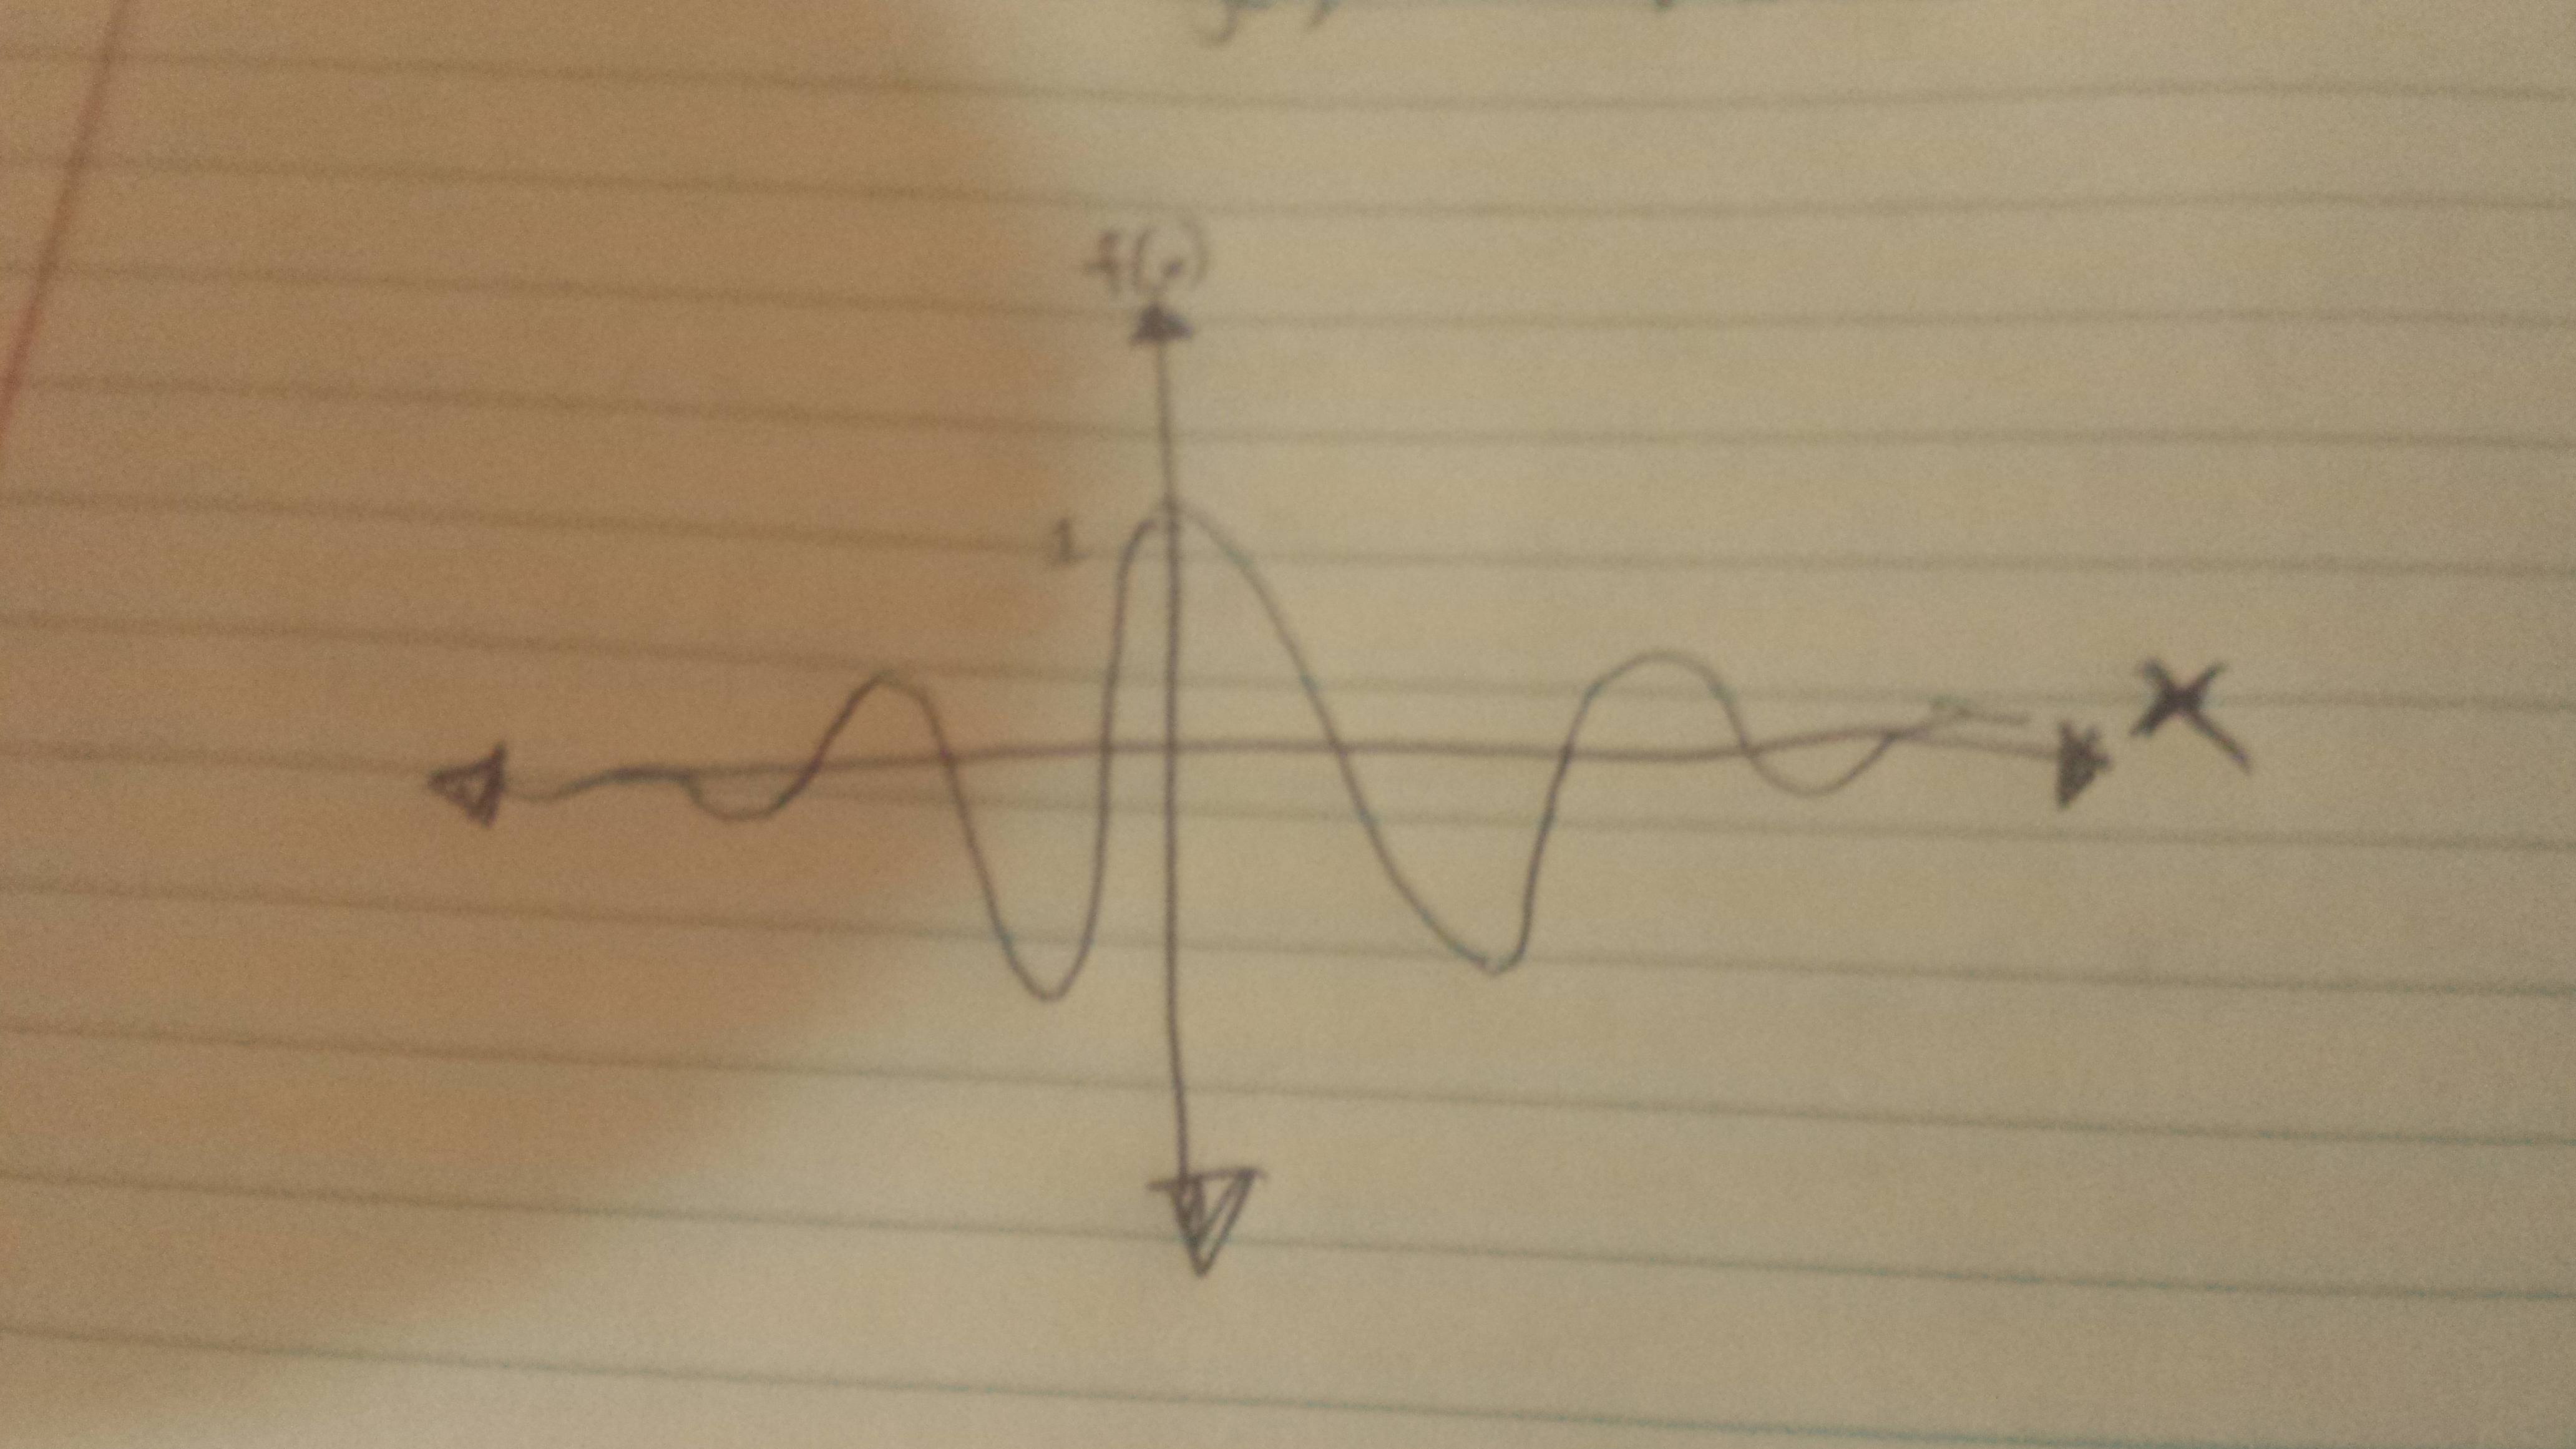
\includegraphics[width=1\textwidth]{img}

    $$\lim_{x \to\ \infty} f(x) = 0$$
    $$\lim_{x \to\ 0^{+}} f(x) = 1$$
    $$\lim_{x \to\ 0^{-}} f(x) = 1$$
    $$\lim_{x \to\ - \infty} f(x) = 0$$
    $$\lim_{x \to\ 0} f(x) = 1$$
  \item [20.7]
    Prove the limit assertions in Exercise 20.3.\\\\
    
    Let $(x_n)$ be some sequence in $(0, \infty)$ with limit $+ \infty$. Since $\lim(\frac{1}{x_n}) = 0$, and since $\sin x$ is bounded between $-1$ and $1$, we know that $\lim(\frac{\sin x}{x_n}) = 0$. The same is clearly true for some sequence in $(-\infty, 0)$.\\

    We can prove that $\lim_{x \to\ 0} f(x) = 1$ with L'Hospital's rule:
    $$\lim_{x \to\ 0} \frac{\sin x}{x} = \lim_{x \to\ 0} \frac{\frac{d}{dx} \sin x}{\frac{d}{dx} x} = \lim_{x \to\ 0} \frac{\cos x}{1} = 1$$
    And from Theorem 20.10, we know that since $\lim_{x \to\ 0} f(x)$ exists, then it must be equal to both $\lim_{x \to\ 0^+} f(x)$ and $\lim_{x \to\ 0^-} f(x)$, which both must be $1$.
  \item [20.16]
    Suppose the limits $L_1 = \lim_{x \to\ a^+} f_1(x)$ and $L_2 = \lim_{x \to\ a^+} f_2(x)$ exist.
    \begin{enumerate}
      \item Show if $f_1(x) \leq f_2(x)$ for all $x$ in some interval $(a,b)$, then $L_1 \leq L_2$.\\\\

        Suppose that $L_1 > L_2$. Let $\epsilon = \frac{L_1-L_2}{2}$. Since $L_1$ exists we know that there must exist some $\delta_1$ such that:
        $$0 < x < a + \delta_1 < b \implies \abs{f_1(x) - L_1} < \epsilon \implies f_1(x) > L_1 - \epsilon \implies f_1(x) > \frac{L_1 + L_2}{2}$$
        Similarly, there must exist some $\delta_2$ such that:
        $$0 < x < a + \delta_2 < b \implies \abs{f_2(x) - L_2} < \epsilon \implies f_2(x) < L_2 + \epsilon \implies f_2(x) < \frac{L_1 + L_2}{2}$$

        So then we know that, for some $\delta = \min \{\delta_1, \delta_2\}$ that:
        $$a < x < a + \delta < b \implies f_2(x) < \frac{L_1+L_2}{2} < f_1(x)$$
        Or that $f_2(x) < f_1(x)$, which is a contradiction.\\

        So we know that $L_1 \leq L_2$.
      \item Suppose that, in fact, $f_1(x) < f_2(x)$ for all $x$ in some interval $(a,b)$. Can you conclude that $L_1 < L_2$?\\\\

        No. Take for example $f_1(x) = x, f_2(x) = 2x$ with the interval $(0,1)$. In this case, $L_1 = L_2 = 0$.
    \end{enumerate}
  \item [20.17]
    Show that if $\lim_{x \to\ a^+} f_1(x) = \lim_{x \to\ a^+} f_3(x) = L$ and if $f_1(x) \leq f_2(x) \leq f_3(x)$ for all $x$ in some interval $(a,b)$, then $\lim_{x \to\ a^+} f_2(x) = L$. This is called the squeeze lemma. (Warning : This is not immediate from Exercise 20.16(a).)\\\\

    Let $\epsilon > 0$. Since $\lim_{x \to\ a^+} f_1(x) = \lim_{x \to\ a^+} f_3(x) = L$, by 20.8, we know there must exist some $\delta_1, \delta_3$ such that:
    $$0 < x < a + \delta_1 \implies \abs{f_1(x) - L} < \epsilon \implies L - \epsilon \leq f_1(x) \leq L + \epsilon$$
    $$0 < x < a + \delta_3 \implies \abs{f_3(x) - L} < \epsilon \implies L - \epsilon \leq f_3(x) \leq L + \epsilon$$
    Let $\delta = \min \{\delta_1, \delta_3 \}$. Then we know that:
    $$0 < x < a + \delta \implies L - \epsilon \leq f_1(x) \leq f_2(x) \leq f_3(x) \leq L + \epsilon$$
    So by 20.8, we know that $\lim_{x \to\ a^+} f_2(x) = L$.
  \item [20.19]
    The limits defined in Definition 20.3 do not depend on the choice of the set $S$. As an example, consider $a < b_1 < b_2$ and suppose $f$ is defined on $(a,b_2)$. Show that if the limit $\lim_{x \to\ a^+} f(x)$ exists for either $S = (a,b_1)$ or $S = (a,b_2)$, then the limit exists for the other choice of $S$ and these limits are identical. Their common value is what we write as $\lim_{x \to\ a^+} f(x)$.\\\\

    Say that $\lim_{x \to\ a^{S_2}} f(x) = L$ for $S_2 = (a,b_2)$. Since every sequence in $S_1 = (a,b_1)$ is in $S_2$, (since the former is a subset of the latter,) from Definition 20.1, we get for free that $\lim_{x \to\ a^{S_1}} = L$.\\

    Now suppose that $\lim_{x \to\ a^{S_1}} f(x) = L$ for $S_1 = (a,b_1)$. Let $(x_n)$ be an arbitrary sequence in $S_2 = (a,b_2)$ with limit $a$. We know that for some $N$, $n > N \implies x_n < b_1$. So the sequence $(y_n) = (x_{n > N})$ is in $S_1$, and so $\lim_{} f(y_n) = L$. Since the limit of a sequence starting from a finite $n$ is the same as the limit of a sequence starting at $1$, $\lim_{n \to\ \infty} f(x_n) = L$, and so $\lim_{x \to\ a^{S_2}} = L$
  \item [21.5]
    Let $E$ be a noncompact subset of $\mathds{R}^k$.
    \begin{enumerate}
      \item Show there is an unbounded continuous real-valued function on $E$.\\\\

        From Heine-Borel we know that $E$ is either not closed or unbounded.\\

        If $E$ is unbounded, then we can construct $f : \mathds{R}^k \rightarrow \mathds{R}^k$, where $f(x) = x$ (identity function). Since $E$ is unbounded, clearly $f$ must be an unbounded function on $E$.\\

        If $E$ is not closed, then its complement is not open, and its closure $E^{-}$ must contain some $x_0$ that is not in $E$. As noted in the hint, we can construct a function $f : \mathds{R}^k \rightarrow \mathds{R}$ where:
        $$f(x) = \frac{1}{d(x,x_0)}$$
      \item Show there is a bounded continuous real-valued function on $E$ that does not assume its maximum on $E$.\\\\

        The function : $g(x) = \frac{\abs{f(x)}}{1 + \abs{f(x)}}$ has supremum of $1$, but cannot possibly achieve it in $E$.
    \end{enumerate}
  \item [21.6]
    For metric spaces $(S_1,d_1)$, $(S_2,d_2)$, $(S_3,d_3)$, prove that if $f : S_1 \rightarrow S_2$ and $g : S_2 \rightarrow S_3$ are continuous, then $g \circ f$ is continuous from $S_1$ into $S_3$.\\\\

    If $g$ is continuous, $\forall s_0 \in S_2, \forall \epsilon_g > 0, \exists \delta_g > 0$ such that:
    $$d_2(s,s_0) < \delta_g \implies d_3(g(s), g(s_0)) < \epsilon_g$$
    And if $g$ is continuous, for $\epsilon_f = \delta_g, \forall s_1 \in S_1, \exists \delta_f > 0$ such that:
    $$d_1(s,s_1) < \delta_f \implies d_2(f(s), f(s_1)) < \delta_g$$

    So then, for some $\epsilon_g > 0$, there exists some $\delta_f, \delta_g$ such that $d_1(s,s_1) < \delta_f \implies d_2(f(s),f(s_1)) < \delta_g \implies d_3(g(s),g(s_0)) < \epsilon_g$, meaning that $f \circ g$ is continuous by definition.
  \item [21.8]
    Let $(S,d)$ and $(S^*, d^*)$ be metric spaces. Show that if $f : S \rightarrow S^*$ is uniformly continuous, and if $(s_n)$ is a Cauchy sequence in $S$, then $(f(s_n))$ is a Cauchy sequence in $S^*$.\\\\

    Let $\epsilon > 0$. Since $f$ is uniformly continuous, there exists some $\delta > 0$ such that $s,t \in S$ and $d(s,t)$ imply $d^*(f(s),f(t)) < \epsilon$.\\

    And since $(s_n)$ is a Cauchy sequence, there must exists some $N$ such that $m,n > N \implies d(s_m,s_n) < \delta \implies d^*(f(s_m), f(s_n)) < \epsilon$. And so by the (metric space) definition of a Cauchy sequence, $(f(s_n))$ is Cauchy.
\end{enumerate}

\end{document}
